\documentclass{ctexart}

\usepackage{amsmath}
\usepackage{amsfonts}
\usepackage{amssymb}
\usepackage{minted}
\usepackage{graphicx}
\usepackage{graphics}
\usepackage{rotating}
\usepackage{subcaption}

\title{Graphics - Final Project}
\author{刘晓义 2017011426}
\date{2020.6}

\setCJKmainfont{Source Han Serif CN}

\begin{document}
\maketitle

\begin{figure}[!ht]
  \centering
  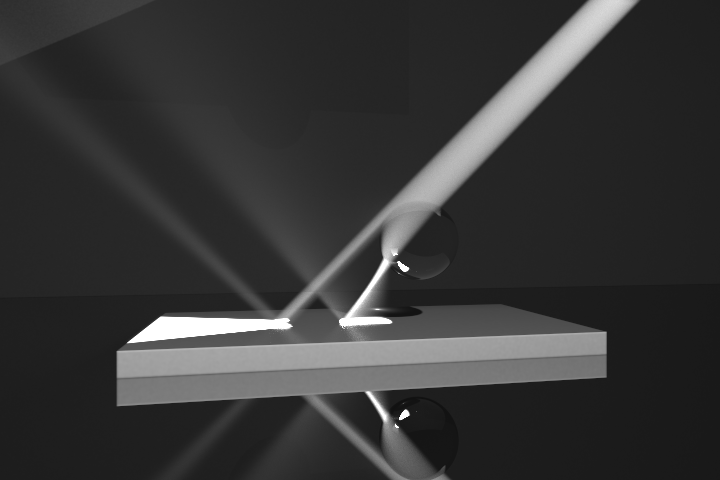
\includegraphics[ width=\textwidth ]{final/volumetric/glass-sphere.png}
  \caption{Glass sphere / volumetric light / Microfacet surface}
  \label{fig:brand}
\end{figure}

\pagebreak

\tableofcontents

\pagebreak

\section{简介}
实现的算法是 SPPM,算法来自 \cite{knaus2011progressive}。实现的语言是 Rust,并未使用渲染或者并行、异构计算框架,使用了社区第三方库帮助向量计算以及用户交互。

\medspace 

支持的其他渲染效果包括
\begin{itemize}
  \item 体积光
  \item 景深
  \item SSAA
  \item Microfacet
\end{itemize}

\medspace

进行的优化包括
\begin{itemize}
  \item BVH 求交加速
  \item 多线程调度器
  \item KD-tree 优化 photon map
\end{itemize}

\section{渲染结果解释}
提交的结果中包含三个目录:
\begin{itemize}
  \item \texttt{refraction} 为了较显著地观察 Specular-Diffuse-Specular 路径渲染细节结果而设计的场景
  \item \texttt{volumetric} 主要为了测试/展示体积光而设计的场景
  \item \texttt{depth} 主要为了测试/展示景深和 Microfacet model 的场景。
\end{itemize}

\subsection{refraction}
场景光源接近在摄像头的正上方,是一个点光源,向其正下方平均辐射光子。

场景内包含三个物体,除了比较简单的金属球、玻璃球以外,比较复杂的物体是一个玻璃砖内嵌了数个不透明的物体。由于有全反射现象,因此可以看到光子在玻璃砖内反射数次之后照明物体,之后再通过折射被摄像头捕捉。

\subsubsection{关于 blocky artifact}
嵌入在玻璃砖内部的球面表面有比较明显的噪声。如果我们输出比较早期的 checkpoint 结果,甚至减小 checkpoint(见图 \ref{fig:refraction-early})可以很明显看到,在迭代次数比较小时,这个球表面的光子分布是非常不均的。这部分光子经历了很多次镜面反射、折射,推测可能是这个原因导致这部分收敛速度远慢于场景中其他的漫反射平面,比如墙体、地面。

注:图 \ref{fig:64} 渲染时光源的设置和最终结果稍有不同:这里的点光源是全方位均匀辐射的,可以从金属球的反光看到不同;并且亮度也有所不同,因此只做示意。

\begin{figure}[ht]
  \centering
  \begin{subfigure}{.45\textwidth}
    \centering
    \includegraphics[width=.8\linewidth]{final/output-64.png}
    \caption{64 次迭代后}
    \label{fig:64}
  \end{subfigure}
  \begin{subfigure}{.45\textwidth}
    \centering
    \includegraphics[width=.8\linewidth]{final/output-1024.png}
    \caption{1024 次迭代后}
    \label{fig:1024}
  \end{subfigure}
  \caption{refraction 场景早期渲染结果}
  \label{fig:refraction-early}
\end{figure}

\subsection{volumetric}
共四个场景,分别表现了光束照射到玻璃砖、玻璃球以及金属球之后产生的体积光效果(图 \ref{fig:brand} 及图 \ref{fig:vol})。glass-sphere-no-reflection 是禁用了所有反射的玻璃球的例子,可以更明显的看到光斑。玻璃砖的例子中可以看到经过内部表面多次反射之后产生了数个光束。

\begin{figure}[ht]
  \centering
  \begin{subfigure}{.3\textwidth}
    \centering
    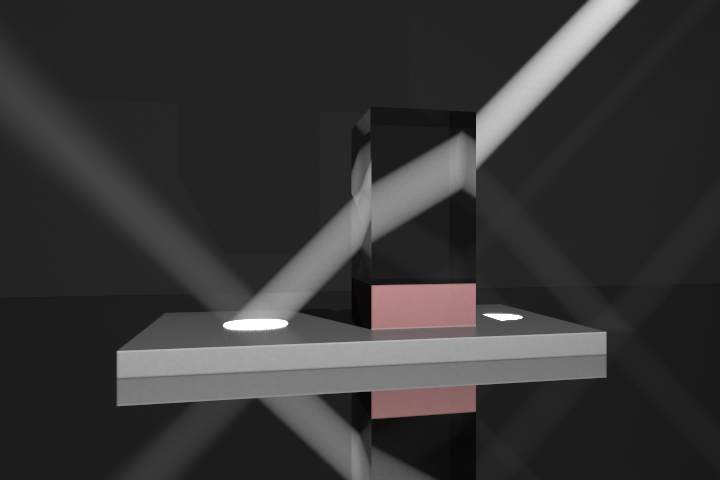
\includegraphics[width=.8\linewidth]{final/volumetric/block.png}
    \caption{玻璃砖}
  \end{subfigure}
  \begin{subfigure}{.3\textwidth}
    \centering
    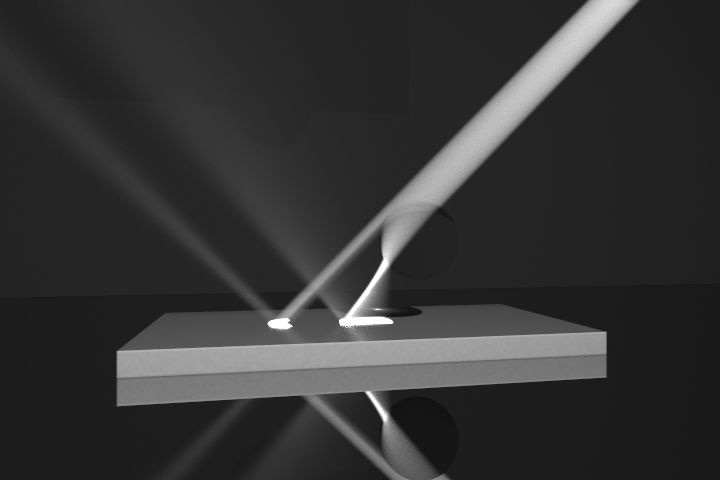
\includegraphics[width=.8\linewidth]{final/volumetric/glass-sphere-no-reflection.png}
    \caption{无反射玻璃球}
  \end{subfigure}
  \begin{subfigure}{.3\textwidth}
    \centering
    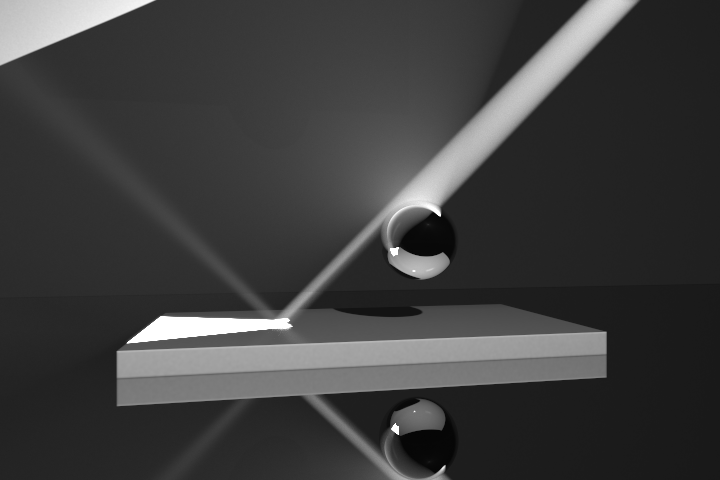
\includegraphics[width=.8\linewidth]{final/volumetric/metal-sphere.png}
    \caption{金属球}
  \end{subfigure}
  \caption{volumetric 场景}
  \label{fig:vol}
\end{figure}

在这三个场景中,除了偏折光线的物体有差别以外,其他布置没有差别:
\begin{itemize}
  \item 拥有两个光源,一个在镜头右后上方,是一个点光源,提供环境光。还有一个是光束。
  \item 地面是有一定吸收的镜面反射,为了体现视线经由反射之后依旧可以看到体积光。从某种意义上而言,这也是 SDS 路径。
  \item 中间的台面具有散射加 Microfacet 表面模型。因此光束经由其反射之后,光束的亮度会降低,并且会丧失集中。同时,视线经由台面表面反射之后,也可以略微看到物体或者光束。
  \item 背景是一个吸收率比较高的完全反射平面,如果观察仔细其实可以看到一些影子,这来自台面和物体遮挡了地面反射的点光源的光。在两个球的例子中,镜头内左上角部分的背景被金属球反射的光线所照亮。
\end{itemize}

\subsubsection{关于收敛速度}
我们在 volumetric 目录下额外给出了玻璃球场景渲染过程的八个checkpoint(除去第二步,这个被我误删了,GG),可以发现,光束部分的收敛速度远慢于场景剩余部分,具体表现是光束中有的像素没有捕捉到光束。在物体的散射表面,Photon map 会帮助获得一个对散射光线较为稳定的估计。虽然介质散射也有类似的行为,对于 SDS 路径中快速获得一个还可以的估计,但是这依赖首先要依赖在做 Distributed ray tracing 的过程中,根据指数分布取步长的时候正好能落到有光子的空间区域内。这导致光束内部的收敛速度要慢很多。体积光的具体实现见第 \ref{sec:vol} 节。
\subsection{depth}
这是一个场景在三个不同的渲染参数下的渲染结果(图 \ref{fig:depth})。渲染参数具体参见第 \ref{sec:options} 节和附录 \ref{sec:cmd}。

墙面和体积光例子中的台面材质相同,因此根据 Microfacet 模型,在淡绿色球体接近的墙面可以看到被染上绿色,地面的阴影内也可以看到在球正下方的亮度要低于球之间的位置。

\begin{figure}[ht]
  \centering
  \begin{subfigure}{.45\textwidth}
    \centering
    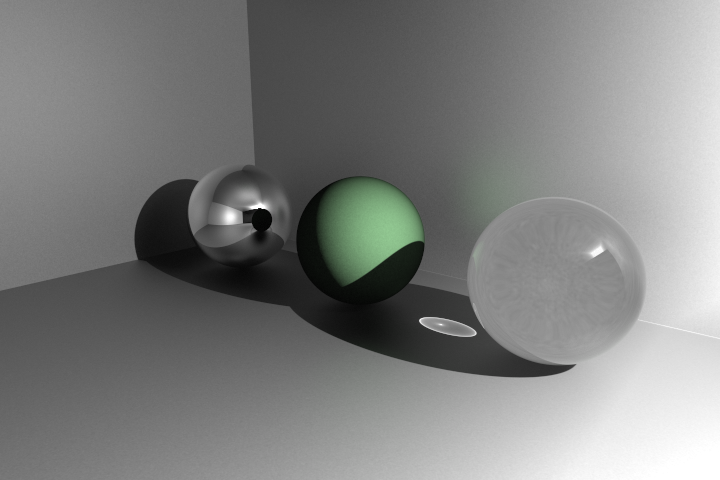
\includegraphics[width=.8\linewidth]{final/depth/none.png}
    \caption{无景深效果}
  \end{subfigure}
  \begin{subfigure}{.45\textwidth}
    \centering
    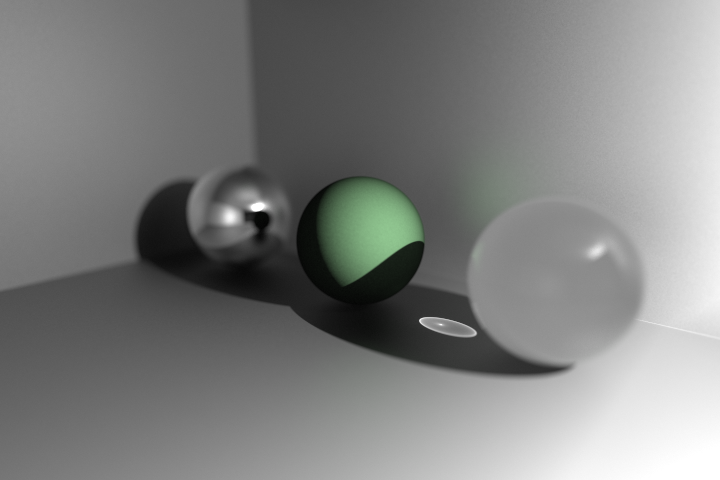
\includegraphics[width=.8\linewidth]{final/depth/2_5.png}
    \caption{弱景深效果}
  \end{subfigure}
  \begin{subfigure}{\textwidth}
    \centering
    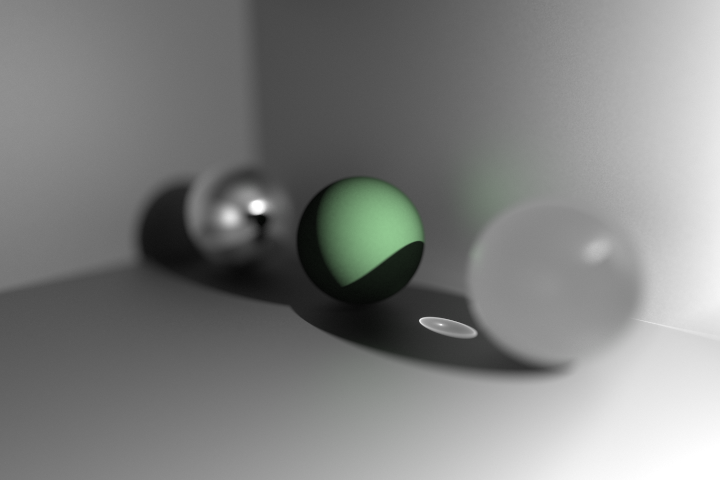
\includegraphics[width=.8\linewidth]{final/depth/5.png}
    \caption{强景深效果}
  \end{subfigure}
  \caption{depth 场景}
  \label{fig:depth}
\end{figure}

\section{实现细节}
\subsection{SPPM}
我们实现的是 \cite{knaus2011progressive} 中的算法,可以省去记录 SPPM 中的局部统计量,使用一个全局统计量就可以达到收敛。这部分代码位于 \texttt{src/renderer.rs} 中的 \texttt{render} 函数中。基本的执行流程为:

\begin{itemize}
  \item 首先,对于每个 Checkpoint,创建 T 个工作线程以及一个调度线程,通过一个 Channel 作为任务队列进行通信。调度线程向 Channel 内推入每轮迭代的编号,以及对应的光子采集半径。
  \item 工作线程轮询任务队列,每次拿到任务后开始执行 PPM 的一轮。
  \begin{itemize}
    \item 首先生成 kdtree 维护的 photon mapping
    \begin{itemize}
      \item 对于每个光子,随机等概率选择一个光源,让其随机发出一个光子。这个光子带有的 Flux 和方向由光源本身的类型和参数决定。
      \item 之后做从光源出发的 path tracing。当求得交点,或发现不存在交点后,需要对体积光做额外处理。具体见第 \ref{sec:vol} 节。
      \item 根据交点处表面的性质,以下两种情况可能出现一个,或者同时出现:
      \begin{itemize}
        \item 表面 BRDF 包含均匀散射分量,那么在 Photon Mapping 中记录这部分散射分量包含的能量。
        \item 表面 BRDF 包含反射分量(包括 Microfacet),或者包含折射分量,那么计算一个可行的反射/折射方向,乘以光通量之后继续做 Path tracing
      \end{itemize}
      \item 根据 Russian roulette 算法决定是否继续下一步。
    \end{itemize}
    \item 对于每个像素,执行从相机出发的 path tracing。相机处生成光线需要考虑景深和超采样。具体见第 \ref{sec:ray-generation} 节。
    \begin{itemize}
      \item 每次产生交点后,同样需要处理体积光。具体见第 \ref{sec:vol} 节。
      \item 根据交点处表面的性质,以下两种情况可能出现一个,或者同时出现:
      \begin{itemize}
        \item 表面 BRDF 包含均匀散射分量,那么从 photon mapping 中收集这一次迭代对应的半径内的光子,通过 Cone filter 之后加和并归一化,乘以视线剩余的通量,加入这一条视线积累的光强中。
        \item 表面 BRDF 包含反射分量(包括 Microfacet),或者包含折射分量,那么计算一个可行的反射/折射方向,乘以通量之后继续做 Path tracing
      \end{itemize}
      \item 根据 Russian roulette 算法决定是否继续下一步。如果决定舍去,那么视线剩余的通量占的比例将会乘回之前积累的光强,以保证无偏。
    \end{itemize}
  \end{itemize}
  \item 调度线程让所有工作线程退出,加和工作线程的所有缓冲区,Gamma 矫正后输出一个图像。
\end{itemize}

\subsection{体积光}
\label{sec:vol}

这部分代码位于 \texttt{src/renderer.rs} 中,标有 \texttt{Volumetric lights} 注释的两个地方,分别对应在 Photon mapping 阶段和在 Distributed ray tracing 阶段对体积光的支持。

实现体积光的时候偷了一个懒:认为任意能量、波段的光子和介质的相互作用概率都是一样的,而且所有的介质和光子的相互作用概率都相同。

如果介质的表面不明显,比如图 \ref{fig:brand} 中的玻璃球,其实会造成比较难以区分介质的问题。所幸即使有了这样的简化,体积光的效果依旧还不错。

在这样的简化下,我们可以只通过一个参数抽象介质和光子相对作用的能力:光子平均自由程 $d$,那么光子在介质中被相互作用掉的距离应该服从指数分布 $Exp(\frac{1}{d})$。这样我们就可以在先求得光线和下一个表面的交点之后,根据这一分布随机决定光子在到达下一个表面前有没有和介质相互作用,在什么位置相互作用了。这一参数通过命令行参数给入,见第 \ref{sec:options} 节。

为了简单实现,体积光部分的实现和表面散射部分的实现有所不同:表面散射部分在光子追踪和视线追踪阶段基本是对称的,当光子经过一个漫反射表面时,仅损失该表面散射的能量。这一考量是为了保证 Photon
map 中的光子数量足够多,减少重复计算。而光子在介质中的散射会直接终止 Path tracing 过程。这是因为为了保证 $d$ 这一参数的估计是有效的,所有的能量都应该在散射中被耗散掉。额外地,光子在介质中被散射后,能量延所有方向平均分布。而在表面散射的能量会和散射的方向有关。

如果希望区分不同介质和光子相互作用的参数,一个可行的方法是在每个表面上带有两侧的参数。在 Path tracing 的过程中维护这一参数,初始化为空气对应的值,每经过一个表面(通过折射)时,更新这一参数即可。

\subsection{视线生成: SSAA 以及景深}
\label{sec:ray-generation}

这部分实现位于 \texttt{src/camera.rs}。生成视线的函数为 \texttt{generate\_ray}。

当生成视线的时候,我们会加入两个随机因素。

首先,均匀生成两个 $\pm 0.5$ 之间的随机数,直接加到像素座标上。这样在大量采样的情况下,可以均匀地完成超采样。

随后,如果以相机作为比喻,我们已经得到了传感器上的一个点。在一个固定焦距下,镜头镜片上每一个点有且仅有一个方向接受到的光线会被聚焦到传感器这个点上。因此我们可以通过“镜片大小”以及“焦距”来抽象景深效果状态。

在生成视线的时候,如果镜片的半径不是 0,随机生成镜头上的一个点,之后可以根据焦距和 FOV 得到这一视线的方向。这样就可以生成景深效果。

\subsection{表面特征:折射以及 Microfacet model}
在我们的实现中,所有的表面都是使用一个相同的 Struct 抽象的:\texttt{src/material/general.rs} 中的 \texttt{General}。

这些表面拥有一下参数衡量其特征:
\begin{itemize}
  \item 散射比例,以及散射通量
  \item 完全反射比例,完全反射以外包括折射和反射的比例,以及折射和反射的通量
  \item Glossy value,用于特征化 Microfacet model(具体而言,每个座标方向上扰动的标准差)
  \item 表面两侧的折射率
\end{itemize}

当光线或者实现到达表面时,散射那部份的光通量由 Photon mapping 算法处理,剩下的折射、反射特征是表面自己需要处理的事情。

决定光线是折射还是反射,首先会受完全反射比例影响。这部分光子会无条件反射,这是用于描述不透光的反射材料表面性质的,例如抛光金属球。

其次,剩余的光子会根据 Schlick's approximation \cite{schlick1994inexpensive} 决定折射和反射的比例。额外的我们可以体现光密介质到光疏介质的全反射。这部分代码位于 \texttt{src/material/general.rs} 中 \texttt{get\_vision\_reflection} 函数中。此处,法向量为折射率 n1 指向 n2 的方向。

如果一个光子或者视线被判断为应该反射,并且存在 Microfacet model 的影响,那么根据表面的参数,随机生成x, y, z 三个方向上的扰动。每个方向上的扰动都遵从正态分布,均值为 0,方差由表面参数决定。这一扰动将会被加到反射光线的方向向量上。这部分代码位于 \texttt{src/material/general.rs} 中 \texttt{generate\_reflection\_ray} 函数中。

\subsection{包围盒和接口抽象}
我们抽象了 \texttt{Object trait} 为光线求交的基本单元。有两类 Struct 实现了这一 Trait:

\begin{itemize}
  \item ObjectGroup,也就是一组对象。ObjectGroup 会额外缓存所有字对象的包围盒,在 ObjectTrait 实现 Object 接口的过程中,进行求交加速。由于 ObjectGroup 可以很自然地构成层次结构,这样也就构成了 BVH。这部分实现位于 \texttt{src/object/mod.rs} 中。
  \item GeometryObject,代表一个几何体再加一个表面材料。几何体同样也是一个 Trait:\texttt{Geometry},也有对应的 GeometryGroup,同样做了包围盒优化。这部分实现位于 \texttt{src/object/geometry/mod.rs} 中。
\end{itemize}

实现 Geometry 的基础几何体有三角形和球面,分别位于 \texttt{src/object/geometry} 目录中各自的文件内。

\section{命令行参数}
\label{sec:options}
程序使用 Rust 的第三方库 \texttt{paw} 和 \texttt{structopt} 处理命令行参数的解析。共支持以下参数:

\begin{itemize}
  \item \texttt{help} 打印帮助
  \item \texttt{height, width} 图像尺寸
  \item \texttt{iter} 迭代次数
  \item \texttt{photon-per-iter} 每轮迭代光子数
  \item \texttt{radius-0} 初始 Photon mapping 半径
  \item \texttt{alpha} 半径减小的参数
  \item \texttt{k} Cone filter 的特征参数
  \item \texttt{checkpoint} 每隔几个迭代保存一个检查点
  \item \texttt{depth} 焦距
  \item \texttt{lens-radius} 对应聚焦镜片的半径
  \item \texttt{mean-dist} 处理体积光中,光子平均自由程
  \item \texttt{volumetric-radius-ratio} 优化体积光收敛速度的参数。具体见第 \ref{sec:vol} 节。
\end{itemize}

\appendix

\section{生成结果所用的指令}
\label{sec:cmd}
我们使用了 Rust 的 Cargo 管理编译,因此直接在项目根目录中执行表 \ref{tbl:cmd} 中的指令就可以尝试对实验结果的复现。

\textbf{注意!}由于我们没有提供选择内置场景的命令参数,可能需要修改部分代码,增删部分注释掉的物体才可以得到一致的结果。\texttt{src/main.rs} 中初始化 Scene 的时候可以选择三个内置 scene 之一,我们将会在以下表格中给出。可能还需要对 \texttt{src/scene.rs} 进行额外的更改。

\begin{sidewaystable}
  \scriptsize
\centering
\begin{tabular}{|c|c|c|}
  \hline
  depth/none.png & focus\_scene & \texttt{cargo run --release  -- -r 0.5 -i 4096 -s 16 -c 1024 -d 75 -l 0 -t 128} \\
  depth/2-5.png & focus\_scene & \texttt{cargo run --release  -- -r 0.5 -i 4096 -s 16 -c 1024 -d 75 -l 2.5 -t 128} \\
  depth/5.png & focus\_scene & \texttt{cargo run --release  -- -r 0.5 -i 4096 -s 16 -c 1024 -d 75 -l 5 -t 128} \\
  \hline
  volumetric/* & volumetric\_scene & \texttt{cargo run --release  -- -r 2.5 -i 8192 -s 16 -c 1024 -t 128 -d 70 -l 0} \\
  \hline
  refraction/* & box\_scene & \texttt{cargo run --release  -- -r 0.5 -i 5120 -s 16 -c 1024 -t 128 -w 1440 -h 960} \\
  \hline
\end{tabular}
\caption{渲染指令}
\label{tbl:cmd}
\end{sidewaystable}

\section{吐槽}
听说 Nori 啥都有,Disney model 也有,Scene loader 也有,大家都在用,很香。

我一直不知道,直到 DDL 当天,所以我什么都没有,甚至连 MPI 都没有,只能全部手写,:cry:

\bibliographystyle{plain}
\bibliography{final}

\end{document}
